%\addcontentsline{toc}{chapter}{Development Process}
\chapter{Design}

%You should concentrate on the more important aspects of the design. It is essential that an overview is presented before going into detail. As well as describing the design adopted it must also explain what other designs were considered and why they were rejected.
%
%The design should describe what you expected to do, and might also explain areas that you had to revise after some investigation.
%
%Typically, for an object-oriented design, the discussion will focus on the choice of objects and classes and the allocation of methods to classes. The use made of reusable components should be described and their source referenced. Particularly important decisions concerning data structures usually affect the architecture of a system and so should be described here.
%
%How much material you include on detailed design and implementation will depend very much on the nature of the project. It should not be padded out. Think about the significant aspects of your system. For example, describe the design of the user interface if it is a critical aspect of your system, or provide detail about methods and data structures that are not trivial. Do not spend time on long lists of trivial items and repetitive descriptions. If in doubt about what is appropriate, speak to your supervisor.
% 
%You should also identify any support tools that you used. You should discuss your choice of implementation tools - programming language, compilers, database management system, program development environment, etc.
%
%Some example sub-sections may be as follows, but the specific sections are for you to define. 

\section{Overall Architecture}
\begin{figure}[H]
	\centering
	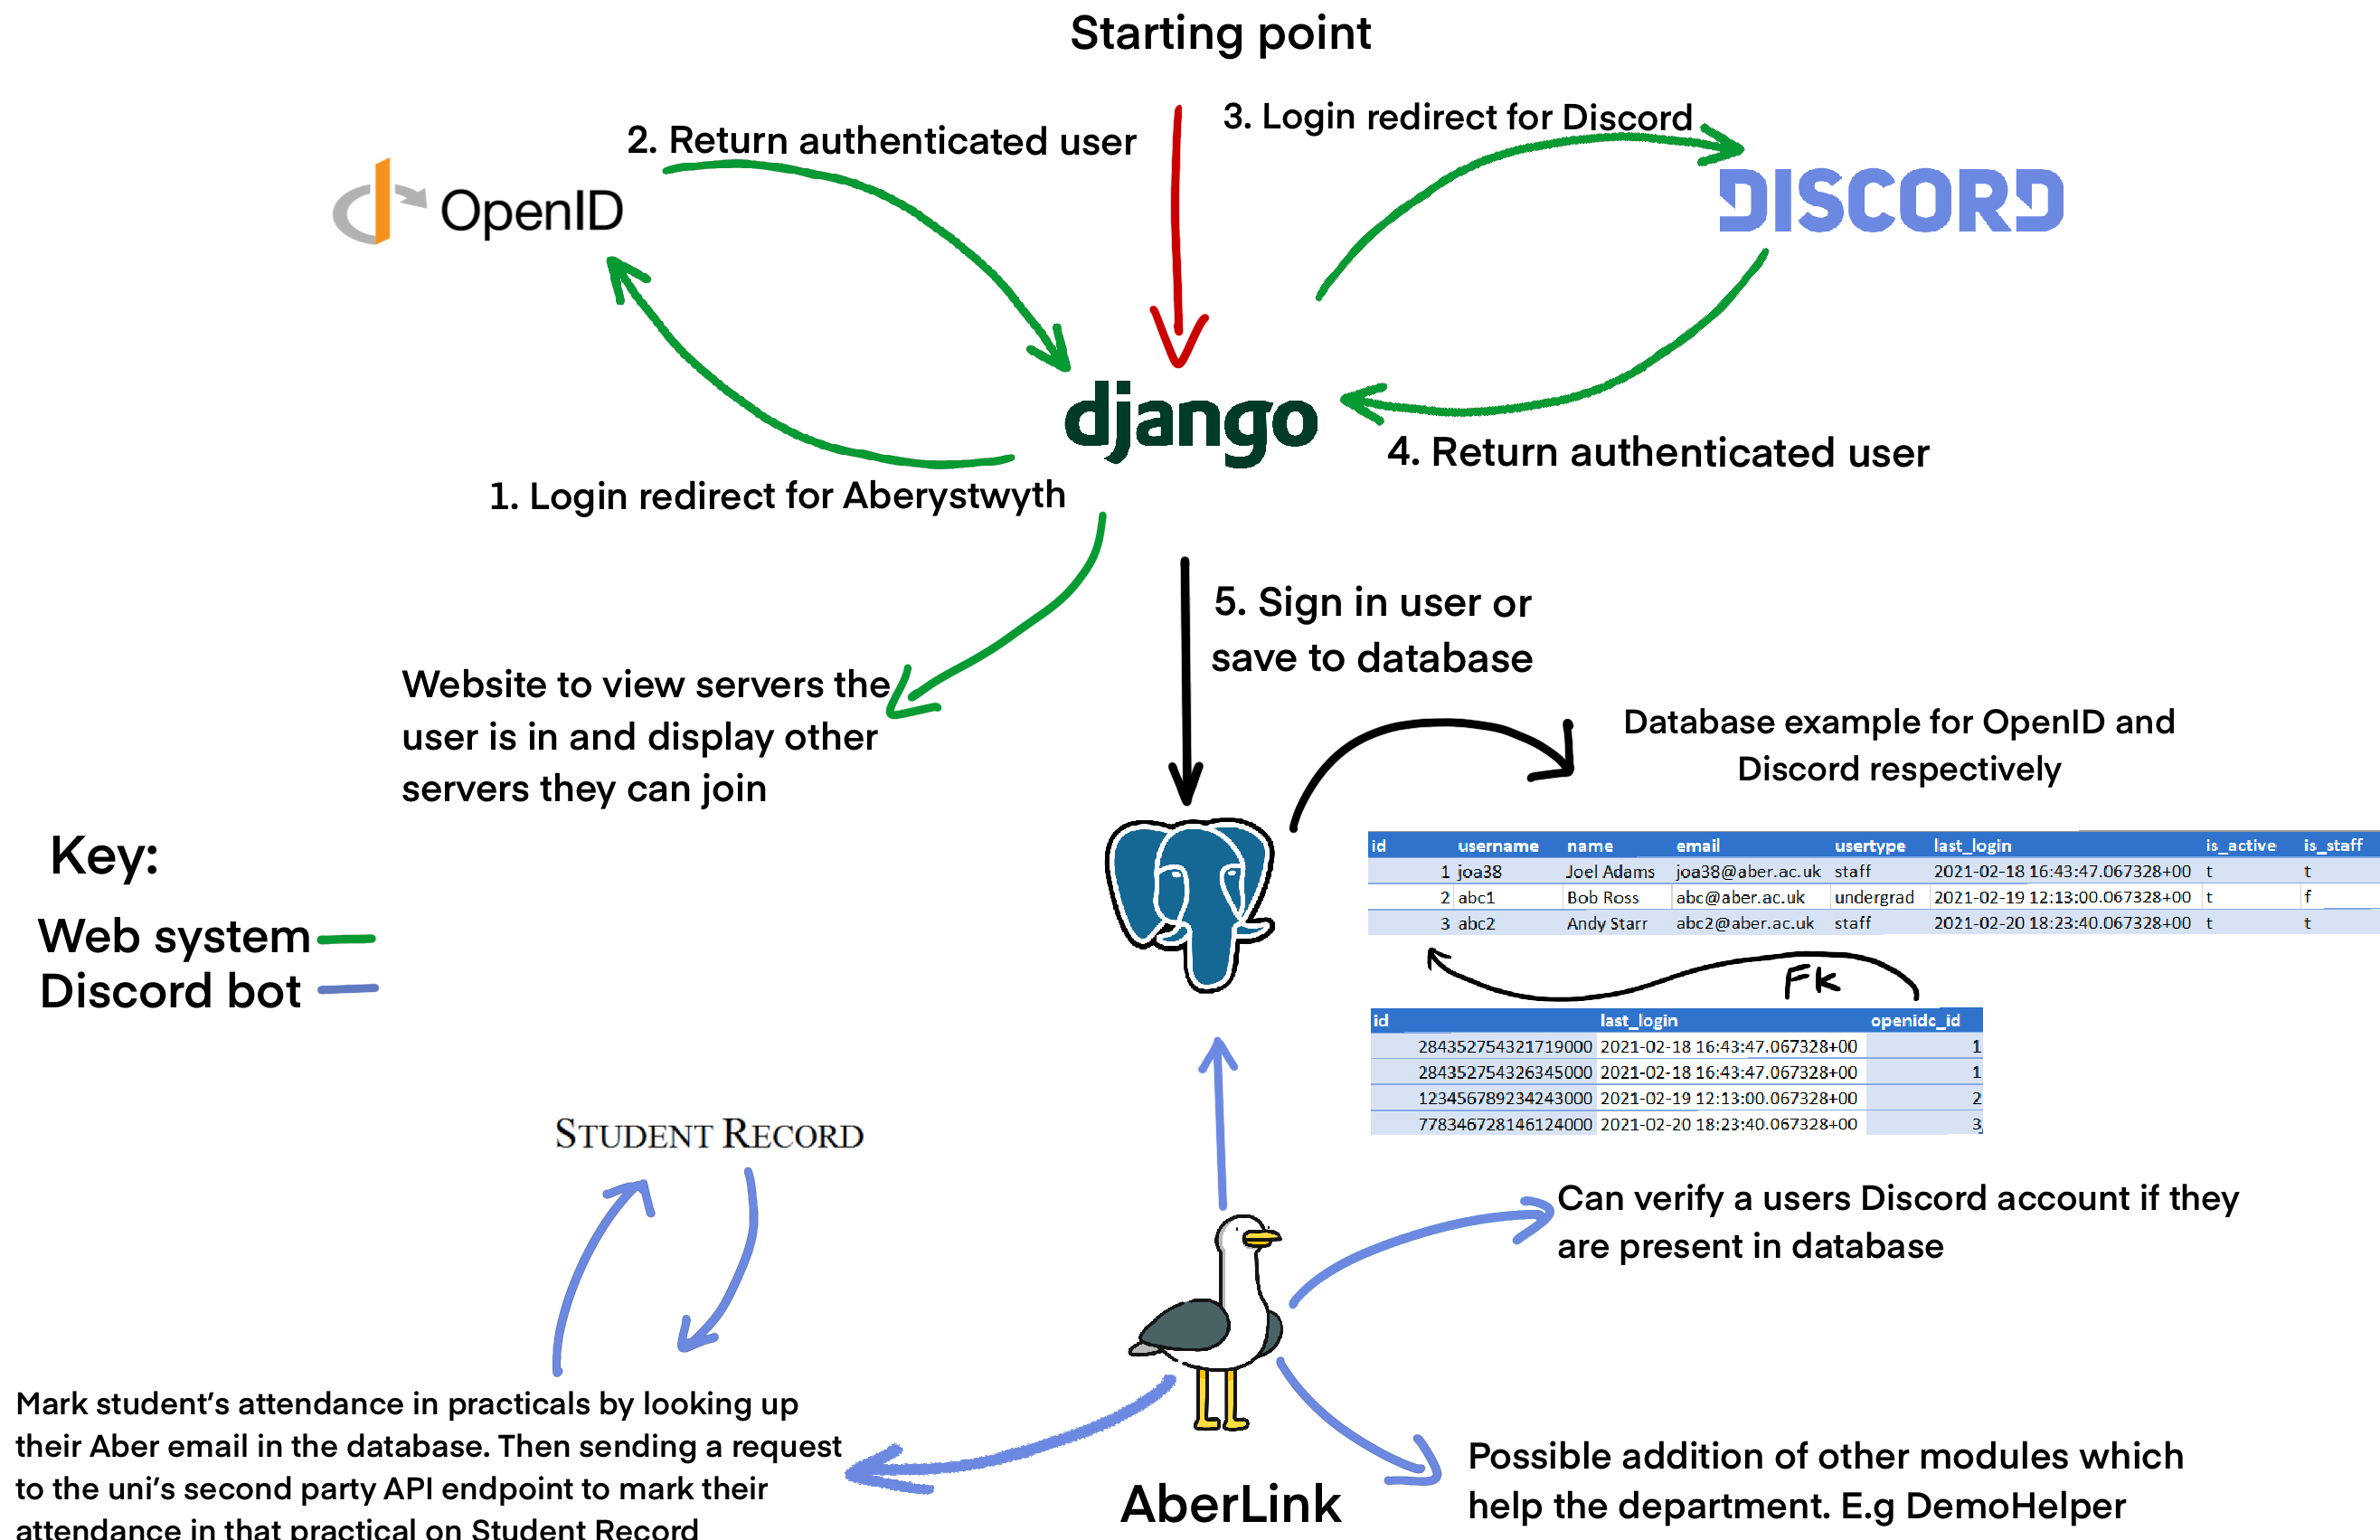
\includegraphics[width=1\linewidth]{Figures/aberlink-flowchart-3}
	\caption{Architecture diagram of the overall system}
	\label{fig:architecture}
\end{figure}

As seen above here is a brief overview of the main components used in this project which are discussed in more detail later on in this document. Below is a list of the main folders and the files contained within them. The folder structure is based largely off of the second year group project folder structure.

\begin{itemize}
	\item \textbf{config} - Describes how to setup the project; a bash script for installing the relevant dependencies, a README.md for manual configuration of the project and example configuration files for Apache2 \cite{apache2}, authentication \cite{libapache2-mod-auth-openidc}, Discord bot and Django \cite{Django}.
	\item \textbf{dev} - Contains the spike work completed throughout this project and some information on errors encountered throughout this project and how they were overcome.
	\item \textbf{docs} - Contains the documents created for this project; including this document, the project outline, the ethics for and the usability form.
	\item \textbf{src} - Contains the source code required to run this project. There are two folders for easier maintainability; a folder for the website and a folder for the Discord bot.
	\begin{itemize}
		\item \textbf{AberLinkAuthentication} - A folder containing all the website resources and the Django \cite{Django} code. It also contains a virtual environment \cite{pipenv} folder that is not stored in git because dependencies update all the time.
		\item \textbf{AberLinkDiscord} - A folder containing the Discord bot. 
	\end{itemize}
\end{itemize}


% Below is a diagram displaying the overall file structure used for the project and was inspired by the second year group project. It has a config folder which describes how to setup the whole project, a folder called dev which contains all of the projects spike work and a folder called docs that contains the latex documents required for this project such as this document. There is also a folder called src that contains two sub folders AberLinkAuthentication and AberLinkDiscord. These two folders are in charge of the website and Discord bot respectively and have been split up as the underlying architecture for each one is vastly different and helps greatly with code maintainability.

% \begin{figure}[H]
% \begin{forest}
% 	for tree={
% 		font=\ttfamily,
% 		grow'=0,
% 		child anchor=west,
% 		parent anchor=south,
% 		anchor=west,
% 		calign=first,
% 		edge path={
% 			\noexpand\path [draw, \forestoption{edge}]
% 			(!u.south west) +(7.5pt,0) |- node[fill,inner sep=1.25pt] {} (.child anchor)\forestoption{edge label};
% 		},
% 		before typesetting nodes={
% 			if n=1
% 			{insert before={[,phantom]}}
% 			{}
% 		},
% 		fit=band,
% 		before computing xy={l=15pt},
% 	}
% 	[aberlink
% 	[config]
% 	[dev]
% 	[docs]
% 	[src
% 	[AberLinkAuthentication]
% 	[AberLinkDiscord]
% 	]
% 	]
% \end{forest}
% \caption{Tree diagram showing overall folder structure}
% \label{fig:architecture-tree}
% \end{figure}

\section{Website Architecture and Design}
\begin{figure}[H]
	\centering
	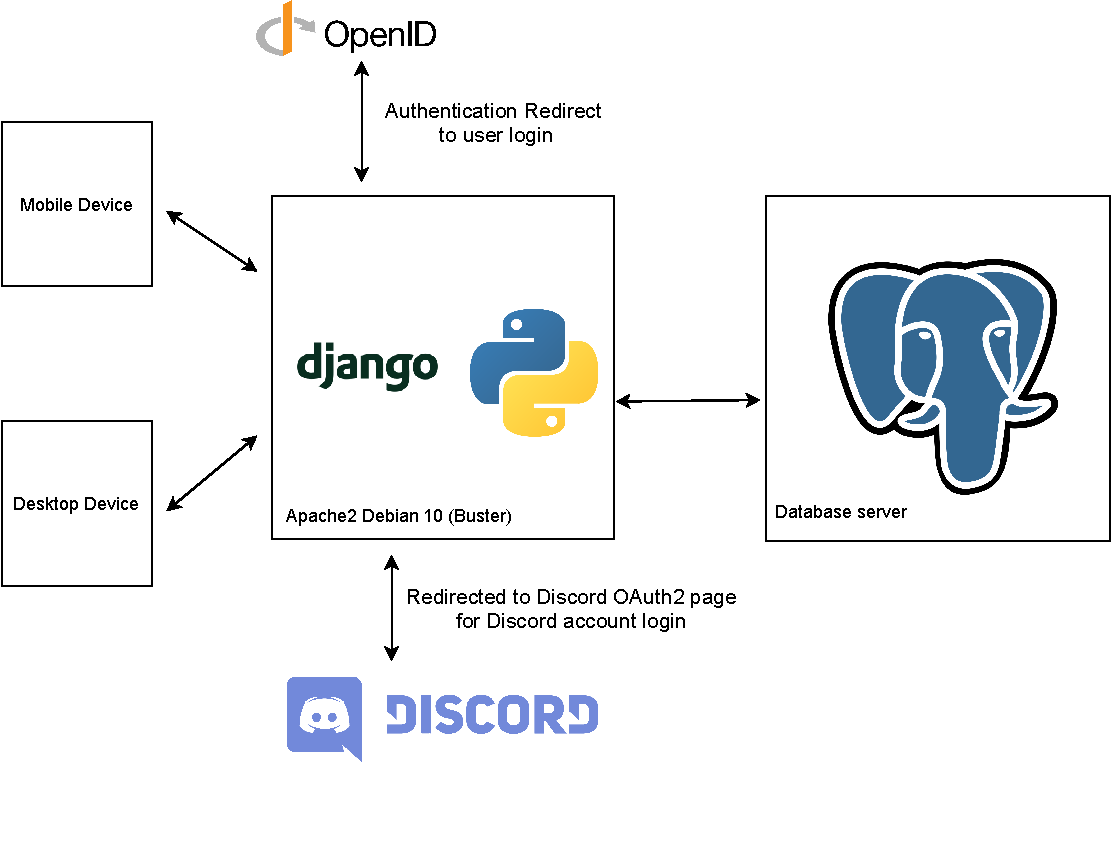
\includegraphics[width=1\linewidth]{Figures/Architecture-website}
	\caption{Architecture diagram of website}
	\label{fig:architecture-web}
\end{figure}

The website is built using the Python framework Django \cite{Django}. This framework has been used to generate a template of the code required and only requires minimal tweaking to setup. When you visit the website you then get redirected to the OpenID Connect \cite{OpenID} authentication framework which helps to prevent unwanted access by users who are not permitted to view the website. Once authenticated the users data is then saved to the database and they can then add Discord accounts by using the button displayed on the screen. This then redirects them to Discord's OAuth2 authentication page and once they have logged in with a discord account then it redirects them back to the my website and saves that information to the database as well. Included below is a flow chart explaining the process works.

\begin{figure}[H]
	\centering
	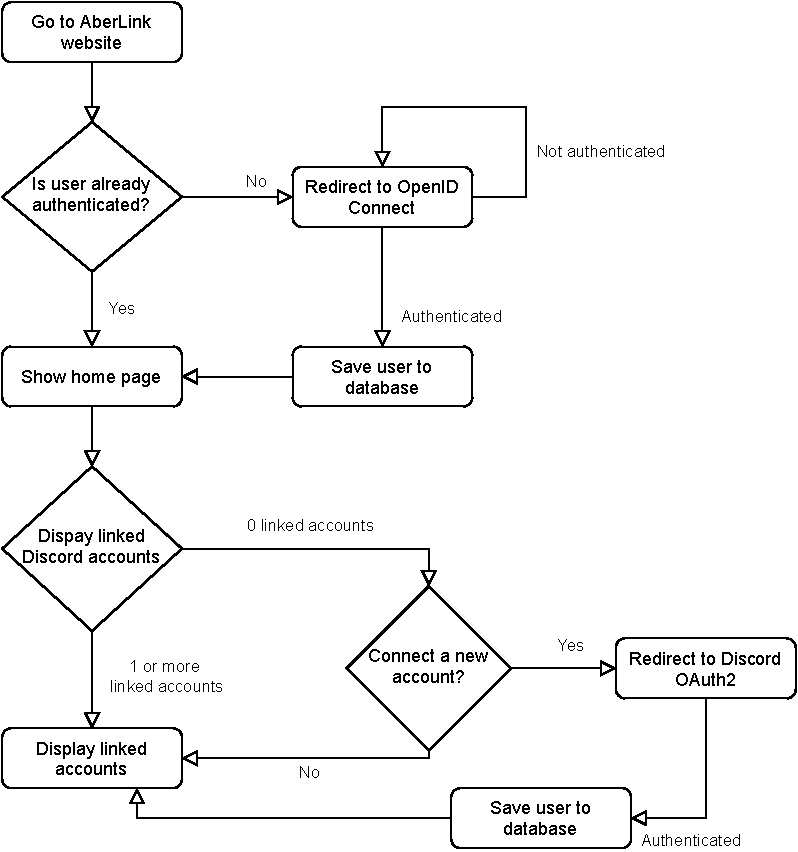
\includegraphics[width=0.8\linewidth]{Figures/website-flowchart}
	\caption{Website flowchart for authentication of accounts and display of user data}
	\label{fig:architecture-web-flow}
\end{figure}

The website can be found here \href{https://mmp-joa38.dcs.aber.ac.uk/}{https://mmp-joa38.dcs.aber.ac.uk/} and is only accessible over VPN.

\section{Discord Bot Architecture and Design}\label{sec2:discord}
\begin{figure}[H]
	\centering
	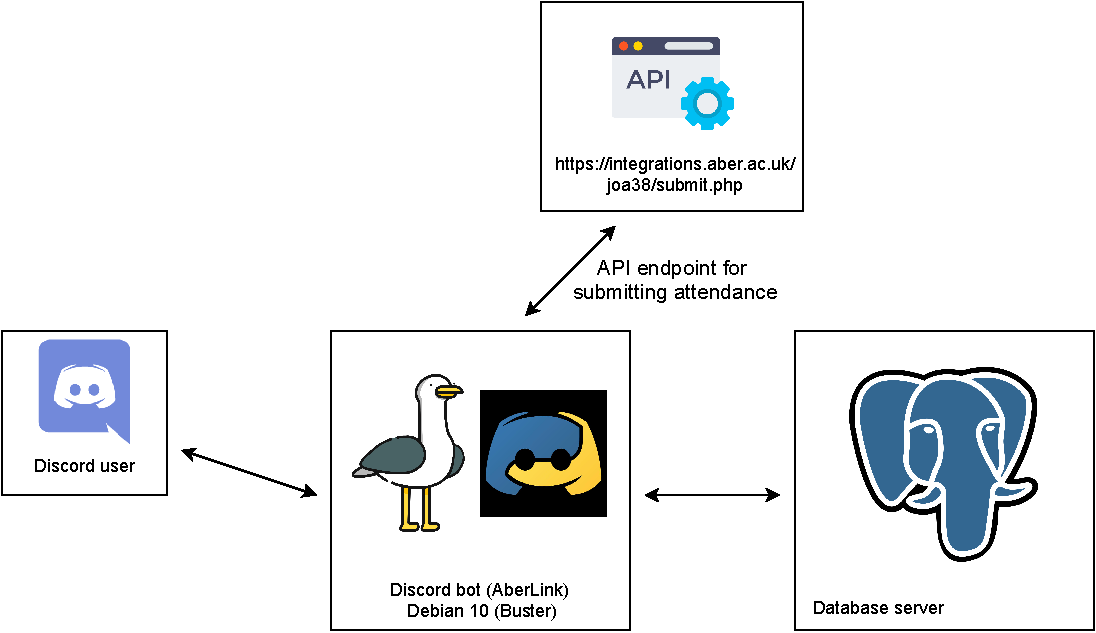
\includegraphics[width=0.9\linewidth]{Figures/Architecture-discord}
	\caption{Architecture diagram of Discord bot}
	\label{fig:architecture-dis}
\end{figure}

The Discord bot (AberLink) is usable through the Discord application available on mobile, desktop and their \href{https://discord.com/app}{website}. AberLink has many commands which can be easily found by typing the `!help' command in Discord on a server where the bot is present or via a direct message to the bot. The basic premise however is that it can access the database to retrieve information about a user but it never saves any information to the database however. The file structure is displayed below.

\begin{figure}[H]
\begin{forest}
	for tree={
		font=\ttfamily,
		grow'=0,
		child anchor=west,
		parent anchor=south,
		anchor=west,
		calign=first,
		edge path={
			\noexpand\path [draw, \forestoption{edge}]
			(!u.south west) +(7.5pt,0) |- node[fill,inner sep=1.25pt] {} (.child anchor)\forestoption{edge label};
		},
		before typesetting nodes={
			if n=1
			{insert before={[,phantom]}}
			{}
		},
		fit=band,
		before computing xy={l=15pt},
	}
	[AberLinkDiscord
	[AberLink.py]
	[Pipfile]
	[.env]
	[cogs
		[\_\_init\_\_.py]
		[db.py]
		[here.py]
		[utilities.py]
		[verify.py]
	]
	]
\end{forest}
\caption{Tree diagram showing Discord file structure}
\label{fig:dis-tree}
\end{figure}

As seen above in the file structure the main file that is used to run the program called AberLink.py, initialising the bot instance and loading all the files from the cogs folder. Discord.py \cite{discord.py} uses a smart system where code is not written into the main file (in this case AberLink.py) but instead broken down into components or `cogs' as they are called here. The .env file is used to to store sensitive variables such as the Discord token required to run the bot and the data used to connect to the database server. This file is also not uploaded to git so the data is never exposed to the wider web and is only stored locally. The Pipfile is used to store the dependencies required to setup the bot such as discord.py \cite{discord.py}, requests \cite{requests}, psycopg2 \cite{psycopg2} and the version of Python required to run the bot. The Pipfile can be initialised using the Python virtual environment pipenv \cite{pipenv}.

\begin{figure}[H]
	\centering
	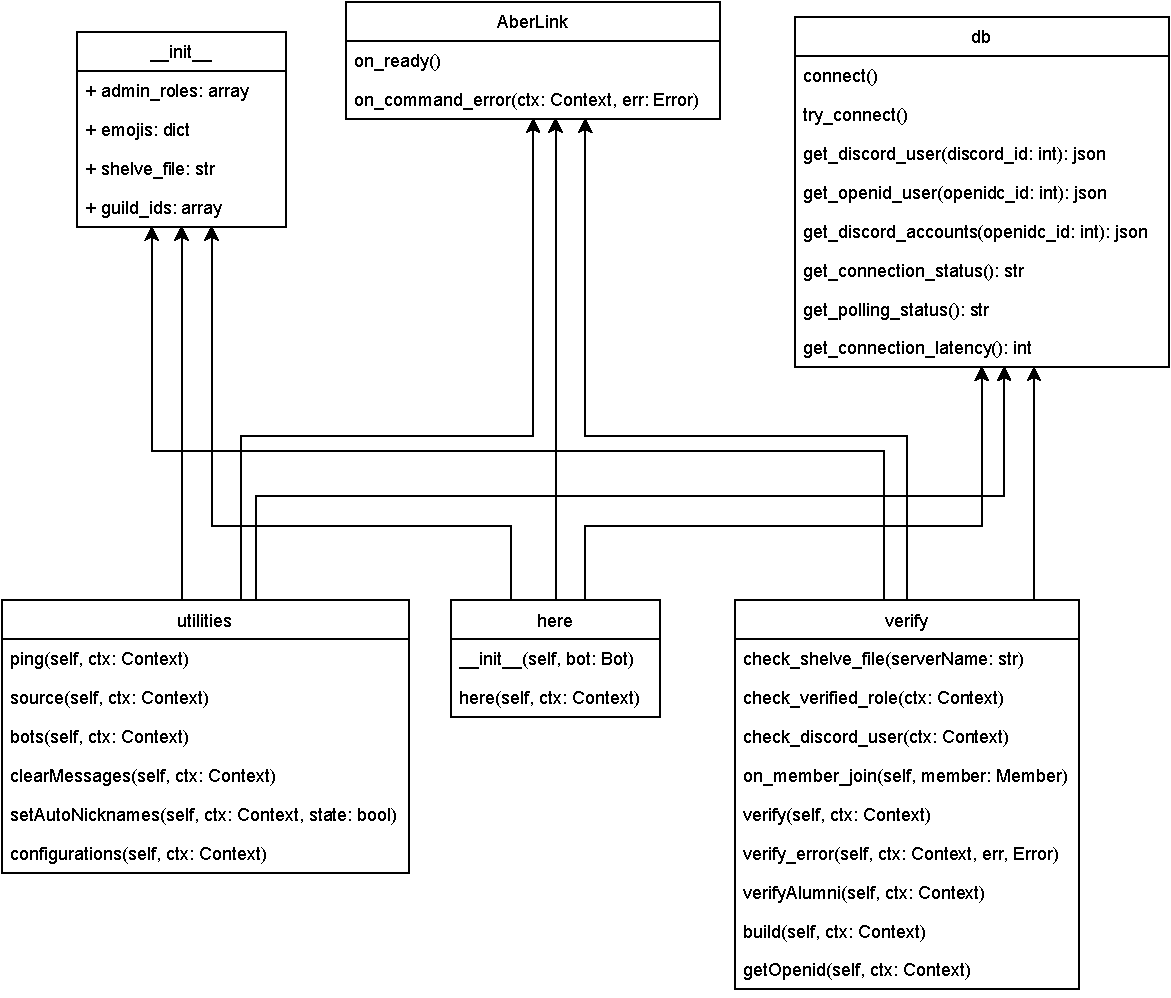
\includegraphics[width=1\linewidth]{Figures/discord-uml}
	\caption{AberLinkDiscord UML diagram}
	\label{fig:discord-uml}
\end{figure}

\subsection{Database Interaction}
Below is a sequence diagram explaining how AberLink connects to the database and sends requests back and forth. It uses the Python library psycopg2 \cite{psycopg2} to connect and send SQL requests back and forth; the details of which can be found in the db.py file. Once connected to the database if an error occurs while making a request then the code executes a function (try\_connection()) to reconnect to the database. Please see Appendix A for more details on psycopg2.
\begin{figure}[H]
	\centering
	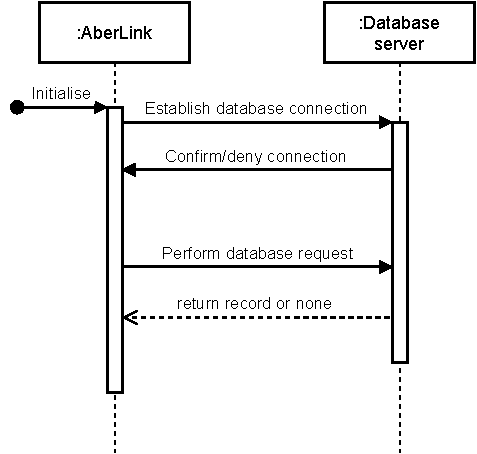
\includegraphics[width=0.5\linewidth]{Figures/aberlink-sequence}
	\caption{Sequence diagram for Discord bot to database}
	\label{fig:architecture-dis-seq}
\end{figure}

\subsection{Discord Commands Interactions}
Discord has two main methods for interacting with Discord bots. The first is by simply typing the command along with the prefix e.g. \verb|!help| would display the information for the help command. This option has been around since the beginning of Discord bots and is a reliable and simple to use method however the end user needs to remember what the commands are to use them. 

The new workaround for this system is to use `slash commands' which are a new feature in Discord that allow the user to type a `/' and Discord then displays a list of available commands that can be used. This feature is incredible and would be very useful to implement if it was not for the current lack of support in relevant libraries. Discord.py \cite{discord.py} does not support the feature at all as it would require an entire library re-write so external libraries have emerged to support this feature such as discord-py-slash-command \cite{discord.py-slash}. These libraries however are currently very early in development and therefore subject to change and restructuring. As this project will be deployed after its creation then we want it to be robust and not break after a new update to the slash commands library.

Despite its infancy, there is basic support for slash commands in AberLink but are commented out. Below is a screenshot to show a working example of the AberLink source command appearing as a Discord `/' command.
\begin{figure}[H]
	\centering
	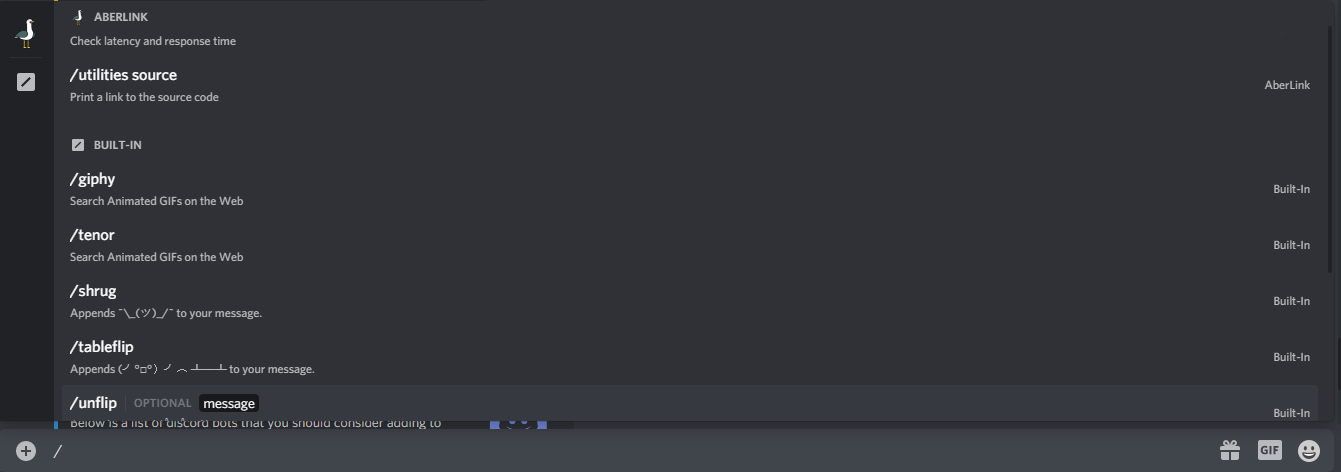
\includegraphics[width=1\linewidth]{Figures/discord-slash.png}
	\caption{Sequence diagram for Discord bot to database}
	\label{fig:architecture-dis-seq}
\end{figure}

\subsection{Complicated Behaviours}\label{sec2:comp-behaviour}
Most of the Discord bot code is relatively straight forward however there is one function in particular that needs some explanation called build() located in AberLinkDiscord/cogs/verify.py. This function and Discord command is used to configure a Discord server for verification. Below is a list of steps that the command executes.

\begin{enumerate}
	\item Begins by simulating that the bot is typing giving the user visual feedback that the command is running as this function usually takes 500ms to 1s.
	\item It then attempts to search for the @everyone role, verify role and \#verify\_channel so that it can update their permissions.
	\item The @everyone role is then stripped of its permissions entirely as it is the only role that is given by default to new joining users. By removing all permissions the new user cannot view any channels.
	\item It then gets the verify role and if it does not exist then it is created and given all the default permissions that @everyone used to have. This basically makes it so that users that have the verified role can do everything that the @everyone role can no longer do.
	\item The bot is then given the verify role so that they can view the server channels and interact with members that have the new verified role.
	\item If the \#verify\_channel does not exist then it is created and a message is pinned to the channel asking users to type !verify to verify their accounts.
	\item The \#verify\_channel is then configured so that users with the @everyone role can view and type in the channel to get verified.
	\item The \#verify\_channel then removes the ability for the verified role to see the channel and therefore sets up a barrier where @everyone and verified can no longer see eachother.
	\item Finally once completed the bot stops typing and sends a message containing all the changes which have been made and the time spent making said changes.
\end{enumerate}

\section{Database design}\label{sec2:database}
Below is the Entity Relationship diagram that describes how the database works. The tables were created in Django which then remodels the psql \cite{psql} database to fit those requirements. 

\begin{figure}[H]
	\centering
	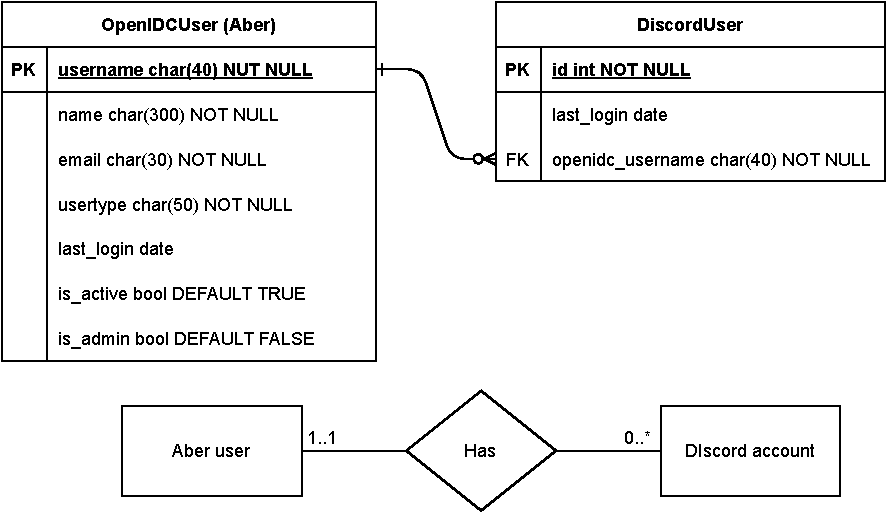
\includegraphics[width=0.8\linewidth]{Figures/database-er-0}
	\caption{Entity relationship diagram for database}
	\label{fig:database-er}
\end{figure}
The \textbf{OpenIDCUser} is the main university account that the user authenticates with and is called so because it uses the OpenID Connect \cite{OpenID} system to authenticate users. The username, name and email are determined from the OpenID Connect response and are all unique. The usertype is also determined by the response and is used to determine if the user will be given administration privileges e.g. if usertype=``staff" then admin=True or if usertype=``student" then admin=False. Due to Django's custom user models it requires that the authenticated account has a is\_active column that is kept true unless the account is marked as deactivated and cannot be used on the website.

The \textbf{DiscordUser} is simple and contains a unique Discord id that is a snowflake; a technology invented by twitter to keep id's unique. It also contains a last\_login date to identify when the account was last authenticated with and lastly a openidc\_id that is a foreign key from the OpenIDCUser's id.

\section{User Interface}\label{sec2:ui}

\subsection{Website}
Before beginning work on the website, some website mock-ups were designed and used as reference when working on the look and feel of the webpages. These mockups were created using the popular design application Figma \cite{figma} and they are located below.
\begin{figure}[H]
	\centering
	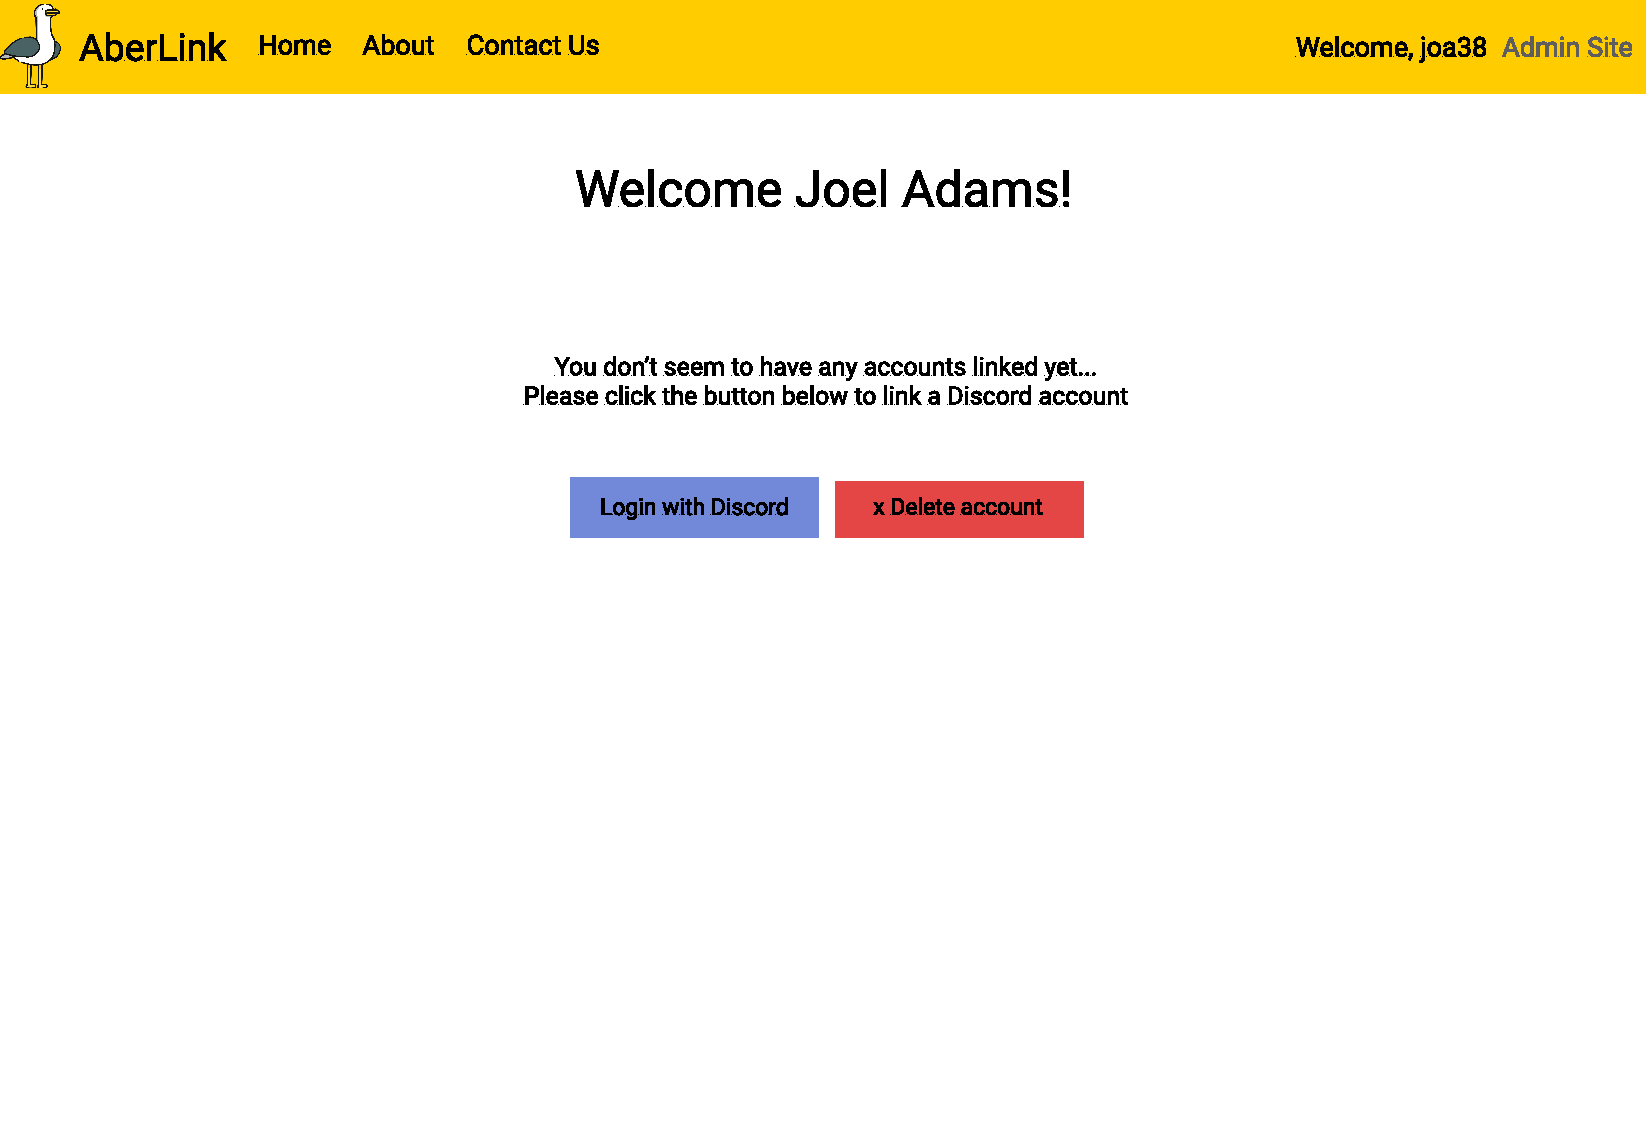
\includegraphics[width=0.8\linewidth]{Figures/AberLink-web-0}
	\caption{Website mock-up for 0 users}
	\label{fig:web-mock-0}
\end{figure}
\begin{figure}[H]
	\centering
	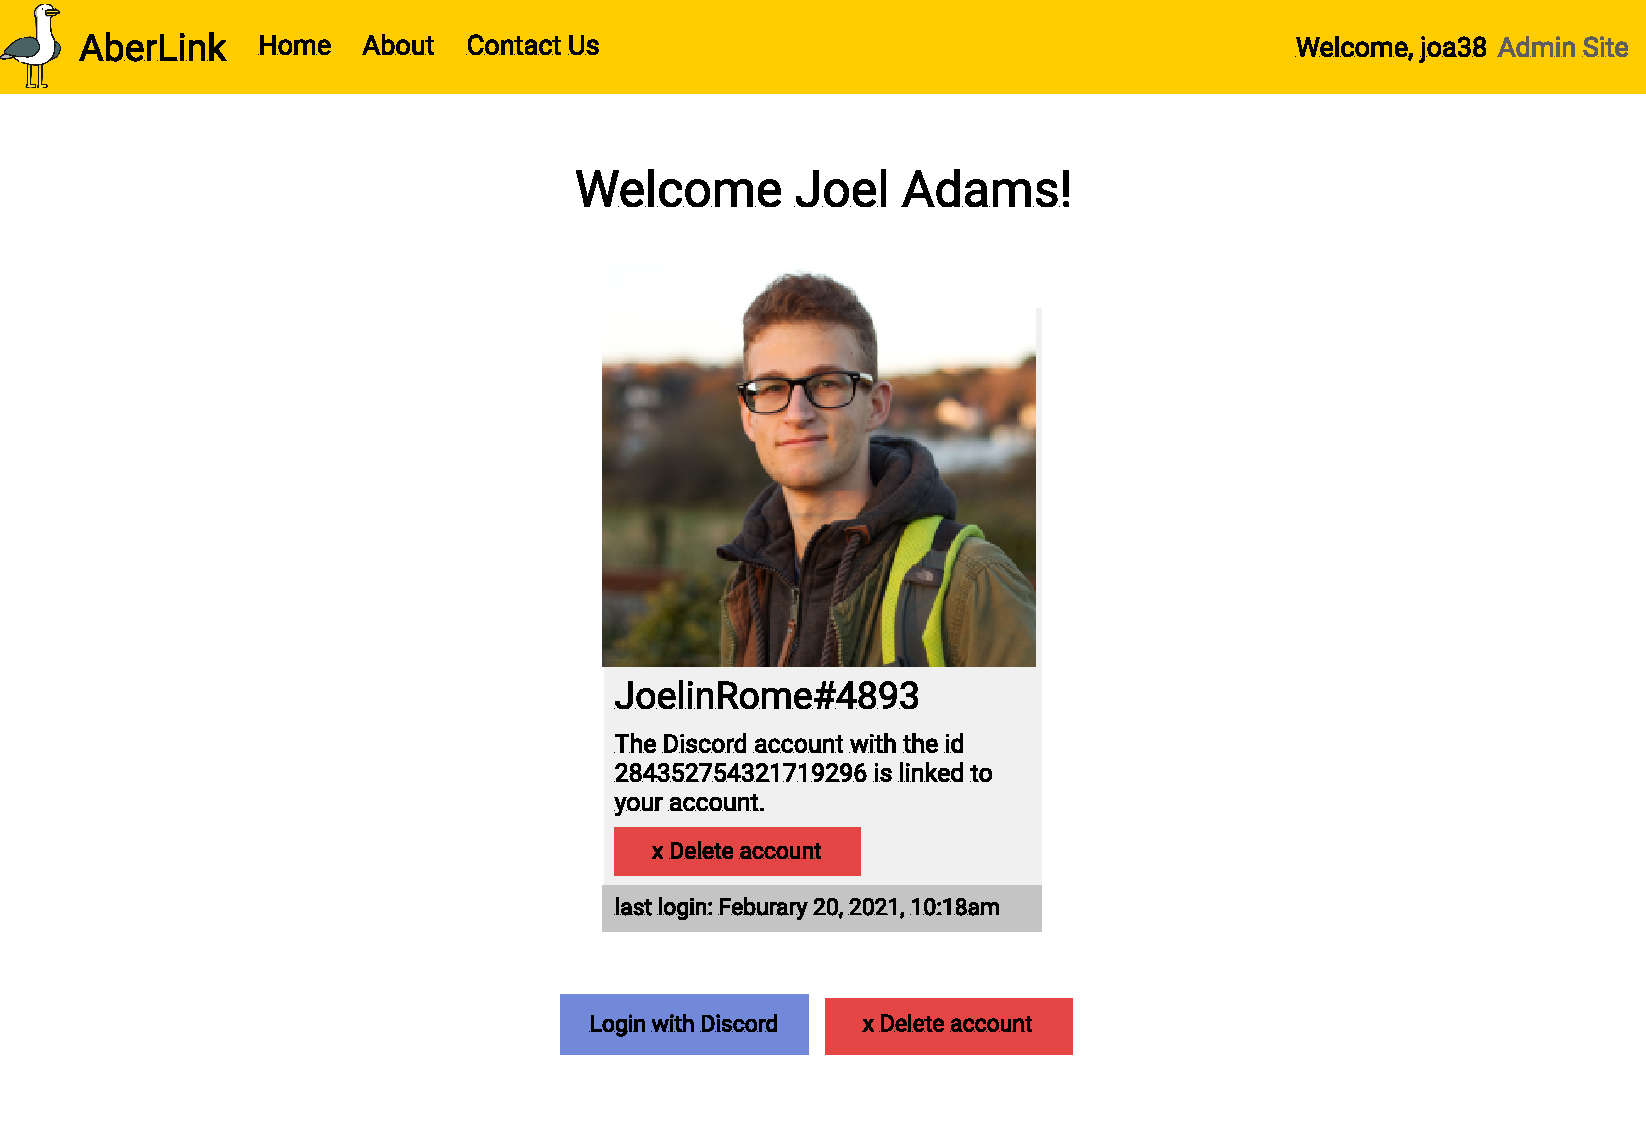
\includegraphics[width=0.8\linewidth]{Figures/AberLink-web-1}
	\caption{Website mock-up for 1 user}
	\label{fig:web-mock-1}
\end{figure}
\begin{figure}[H]
	\centering
	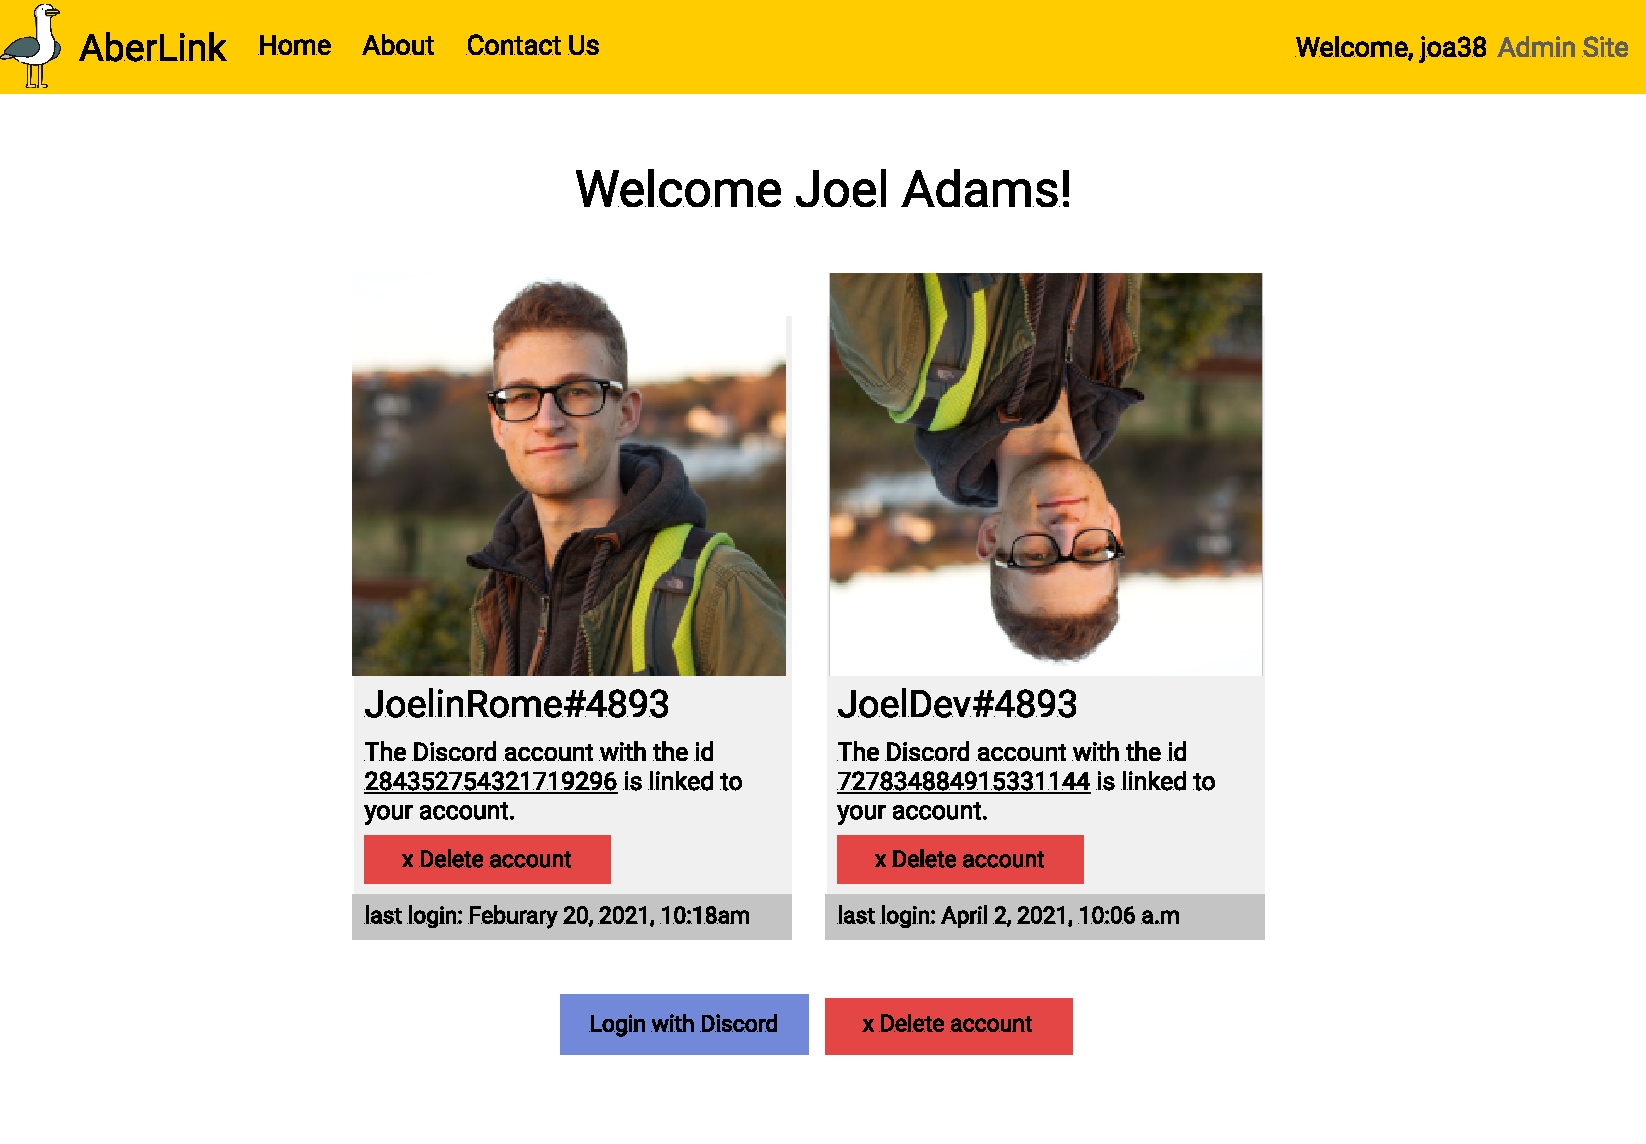
\includegraphics[width=0.8\linewidth]{Figures/AberLink-web-2}
	\caption{Website mock-up for 2 users}
	\label{fig:web-mock-2}
\end{figure}


\subsection{Discord bot}
Discord provides its own interface for Discord bots and does not vary much from the regular interface provided to users. Discord bots however have the additional feature of being able to use Embeds which contain far better formatting than regular messages and are used extensively throughout AberLink. Below are some examples of the output of bot commands that use Discord Embeds.
\begin{figure}[H]
	\centering
	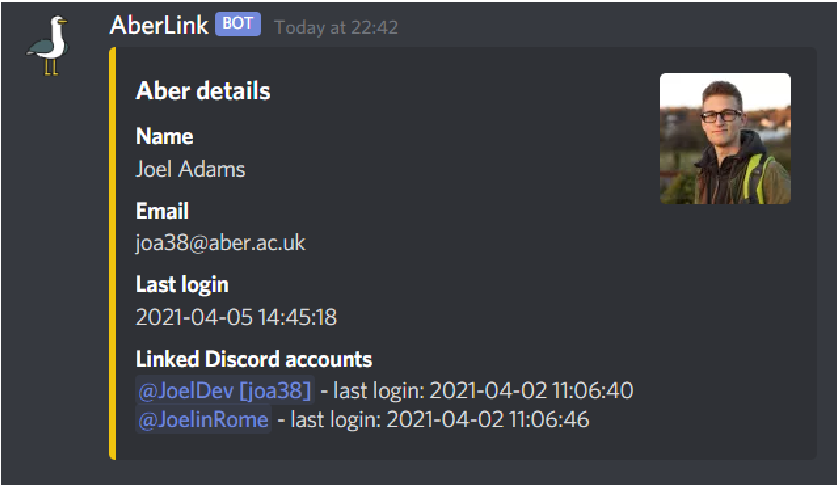
\includegraphics[width=0.8\textwidth]{Figures/test-2}
	\caption{Discord Embed example for getting users information}
	\label{fig:dis-go}
\end{figure}
\begin{figure}[H]
	\centering
	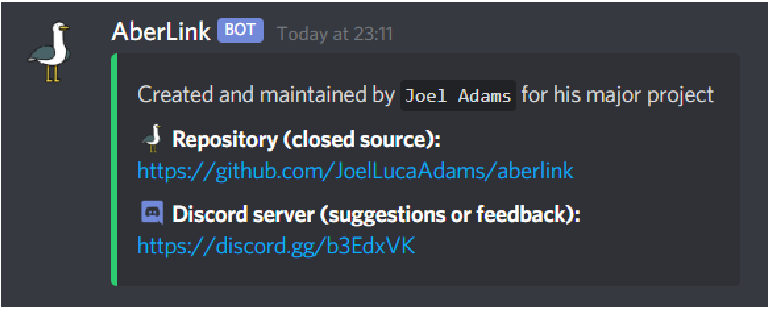
\includegraphics[width=0.8\textwidth]{Figures/test}
	\caption{Discord Embed example for source command}
	\label{fig:dis-source}
\end{figure}

\section{Version Control System and IDE}

Over the last year of working in Python I have used JetBrains Python IDE PyCharm \cite{pycharm} to code my Python projects but recently switched to Visual Studio Code \cite{vsc} due to the amount of extensions it supports and the versatility it has. It was chosen because it has extensions for querying a psql \cite{psql} database, compile Python programs, use virtual environments and write LaTeX documents like this one. It also allows you to remotely connect to a server or container over SSH which is very useful as the majority of the project was developed on a Linux (Debian 10 Buster \cite{debian}) container located in the university \href{https://mmp-joa38.dcs.aber.ac.uk/}{https://mmp-joa38.dcs.aber.ac.uk/}. PyCharm does not support this feature and was one of the key features why it was ruled out for this project.

GitLab was chosen for the version control system using the instance provided by the university to store my code \href{https://gitlab.dcs.aber.ac.uk/}{https://gitlab.dcs.aber.ac.uk/}. Mirroring has also been setup so that the project is copied to another repository called aberlink on my primary GitHub account in case of emergencies or loss of data. Included below is an example of the commits that are made to the repository.
\begin{figure}[H]
	\centering
	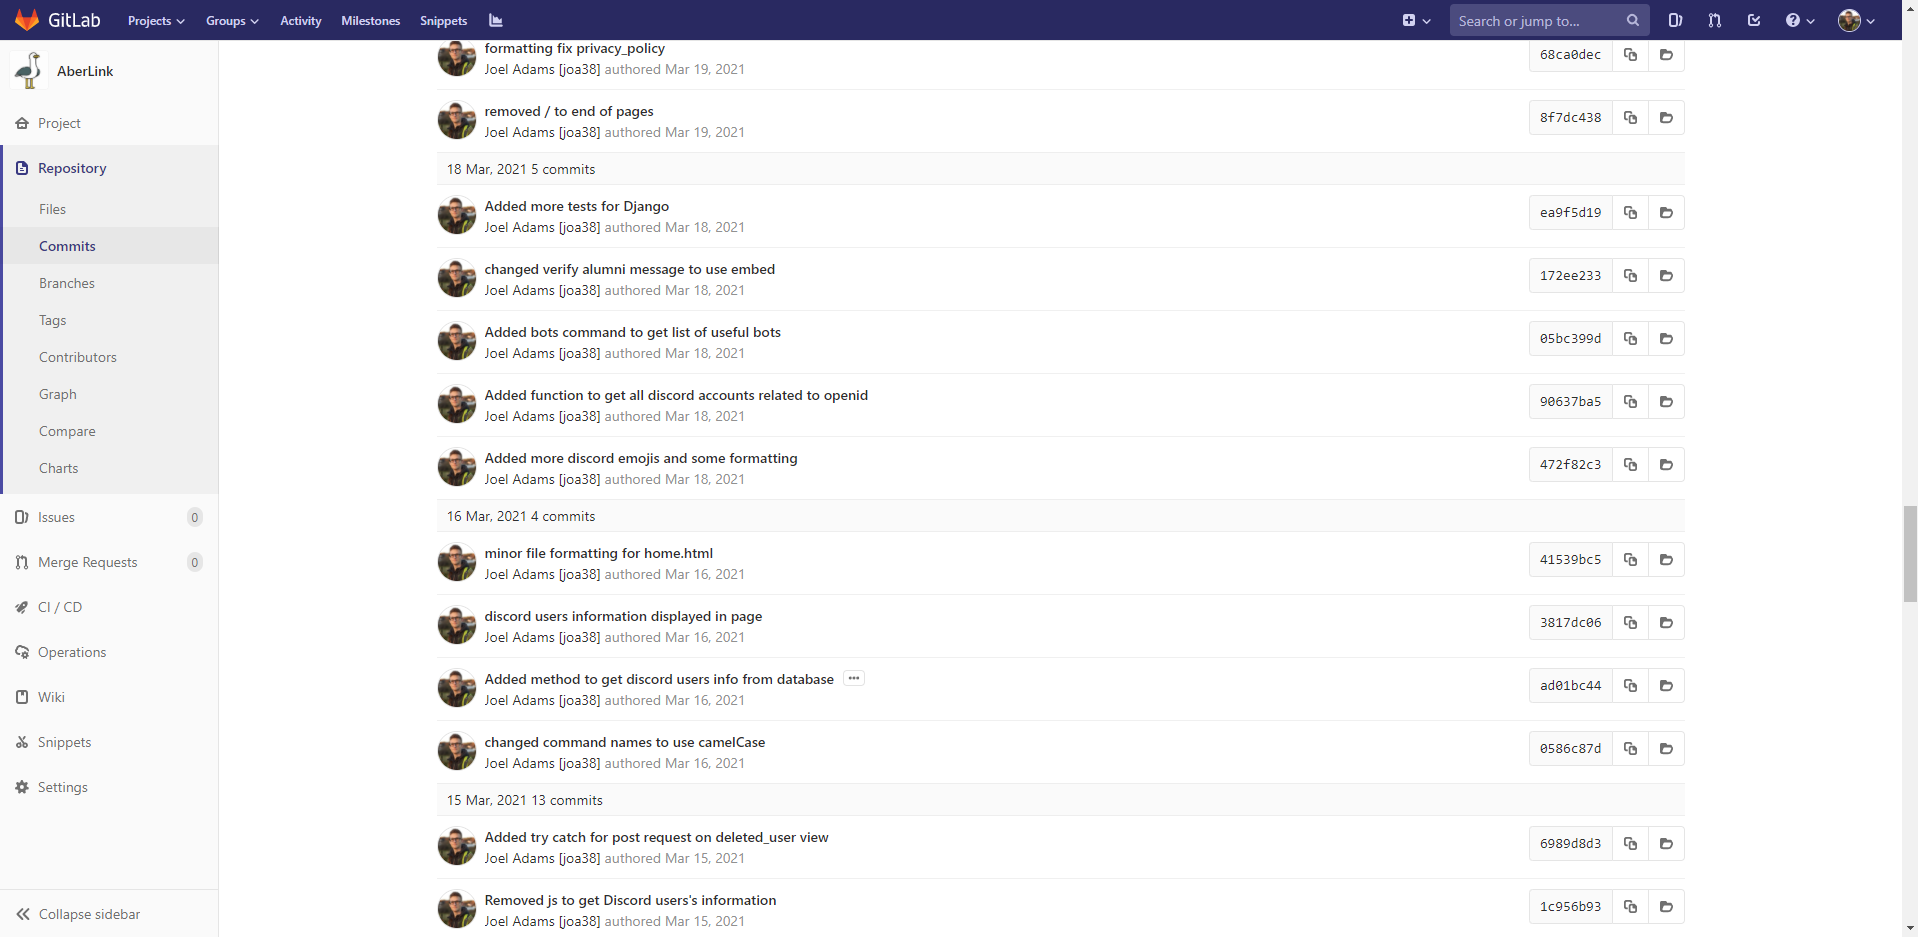
\includegraphics[width=1\textwidth]{Figures/gitlab.png}	
	\caption{Example of GitLab repository commits}
	\label{fig:gitlab}
\end{figure}
